\documentclass[hyperref={pdfpagelabels=false}]{beamer}

\usepackage{xeCJK}
\setCJKmainfont[AutoFakeSlant=0.25]{Noto Sans Mono CJK SC}
\setCJKsansfont[AutoFakeSlant=0.25]{Noto Sans Mono CJK SC}
\setCJKmonofont[AutoFakeSlant=0.25]{Noto Sans Mono CJK SC}

\usepackage{python}
\usepackage{lmodern}
\usetheme{Madrid}
\usecolortheme{dolphin}
\title{科技论文写作文献检索}  
\subtitle{联邦学习中的通信优化}
\author{ 叶茂青 \quad 王珺 } 
\date{\today} 
\begin{document}
\begin{frame}
\titlepage
\end{frame} 

\begin{frame}
	\frametitle{总览}
	\tableofcontents
\end{frame} 

\section{介绍}
\begin{frame}
	\tableofcontents[currentsection]
\end{frame} 

\begin{frame}
	\frametitle{联邦学习的定义}
	\begin{itemize}
		\item 联邦学习的数学模型被McMahan et al.定义为$$\min _{w} F(w), \text { where } F(w):=\sum_{k=1}^{m} p_{k} F_{k}(w)$$
		\item 通俗来说,就是多个客户端通过中心服务器的协调合作解决一个机器学习问题
	\end{itemize}
	\begin{figure}
		\centering
		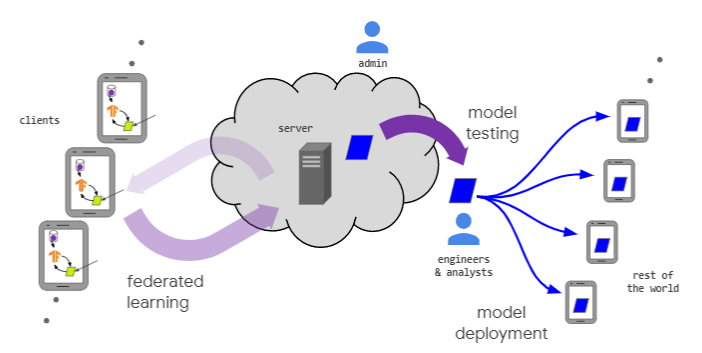
\includegraphics[width=\textheight]{1.png}
	\end{figure}
\end{frame}


\begin{frame}
	\frametitle{联邦学习的特点}
	\begin{itemize}
		\item 客户端数据保存在本地,不会上传给服务器
		\item 数据不满足IID(独立同分布)假设
		\item 客户端的处理能力,带宽是有限的,且不一定可靠
	\end{itemize}
\end{frame}



\section{文献搜索}
\begin{frame}
	\tableofcontents[currentsection]
\end{frame} 
\begin{frame}
	\frametitle{寻找综述论文}
	\begin{figure}
		\centering
		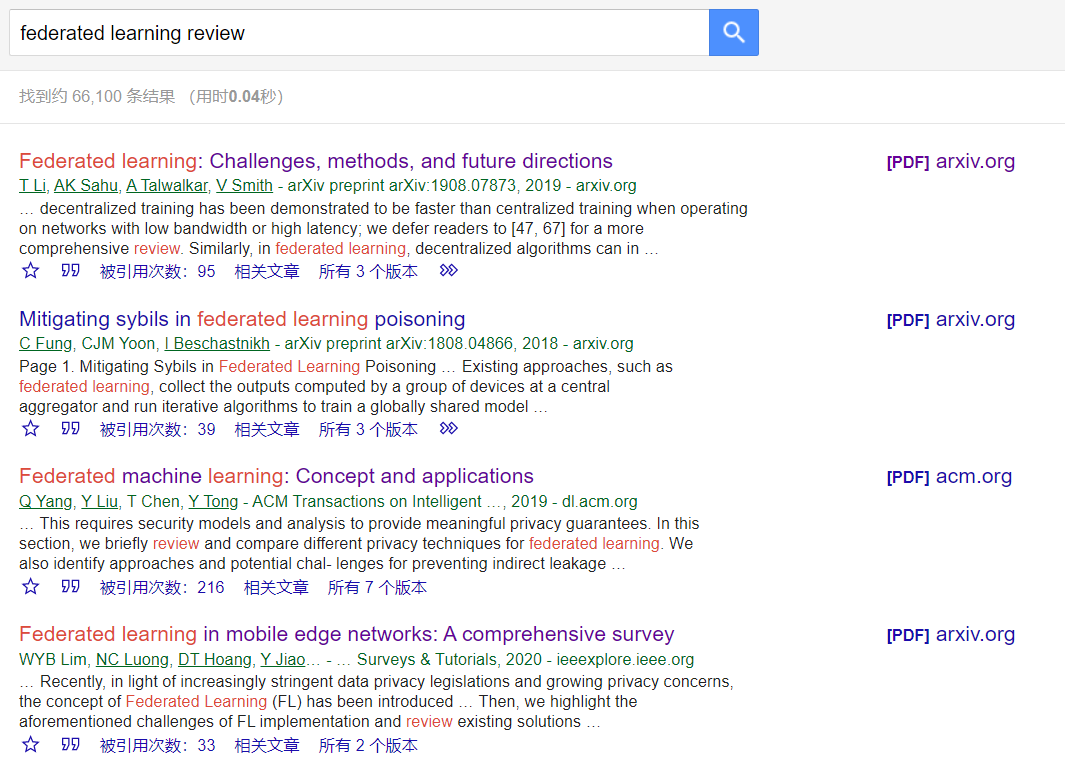
\includegraphics[width=\textheight]{2.png}
	\end{figure}
\end{frame}

\begin{frame}
	\frametitle{寻找综述论文}
	\begin{figure}
		\centering
		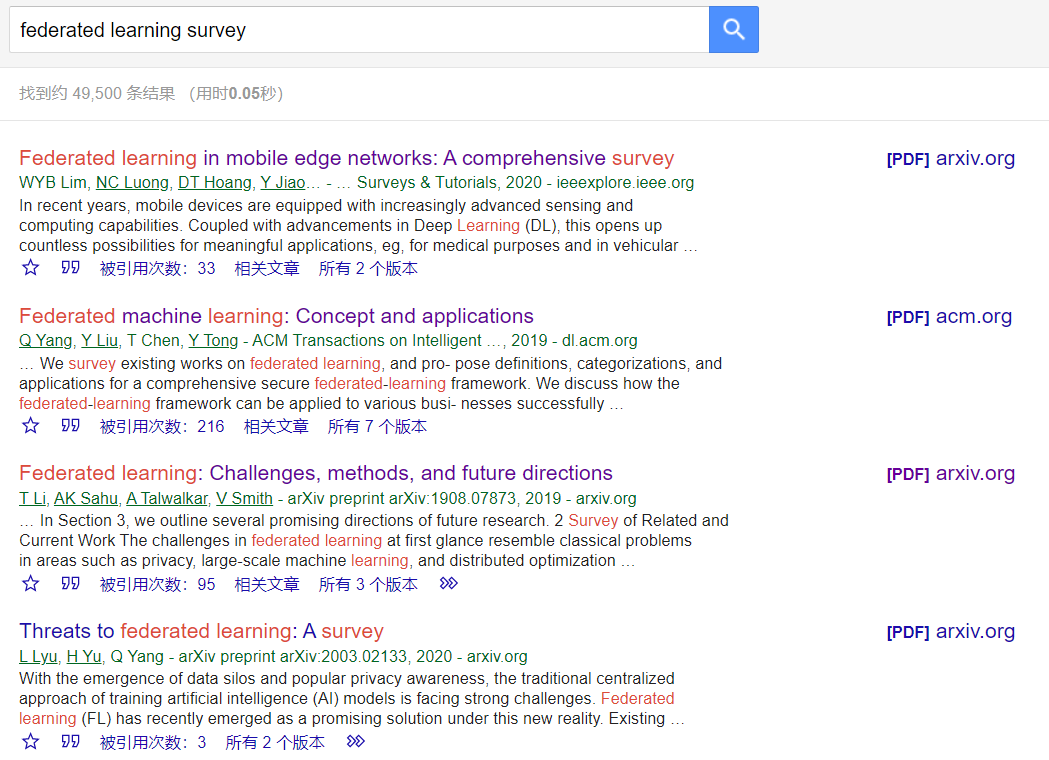
\includegraphics[width=\textheight]{3.png}
	\end{figure}
\end{frame}

\begin{frame}
	\frametitle{了解定义及相关问题}
\end{frame}


\begin{frame}
	\frametitle{细化领域}
\end{frame}



\section{文献分类}
\begin{frame}
	\tableofcontents[currentsection]
\end{frame} 
\begin{frame}
	\frametitle{确定分类标准}
\end{frame}



\section{未来方向}
\begin{frame}
	\tableofcontents[currentsection]
\end{frame} 
\begin{frame}
	\frametitle{结论}

\end{frame}



\begin{frame}{}
	\centering \Huge
	\emph{Thank You!}
\end{frame} 

\end{document}

